\chapter{Diagrammes de fonctionnement}

\section{Fonctionnalités de l'application}

\begin{figure}[h]
  \center
  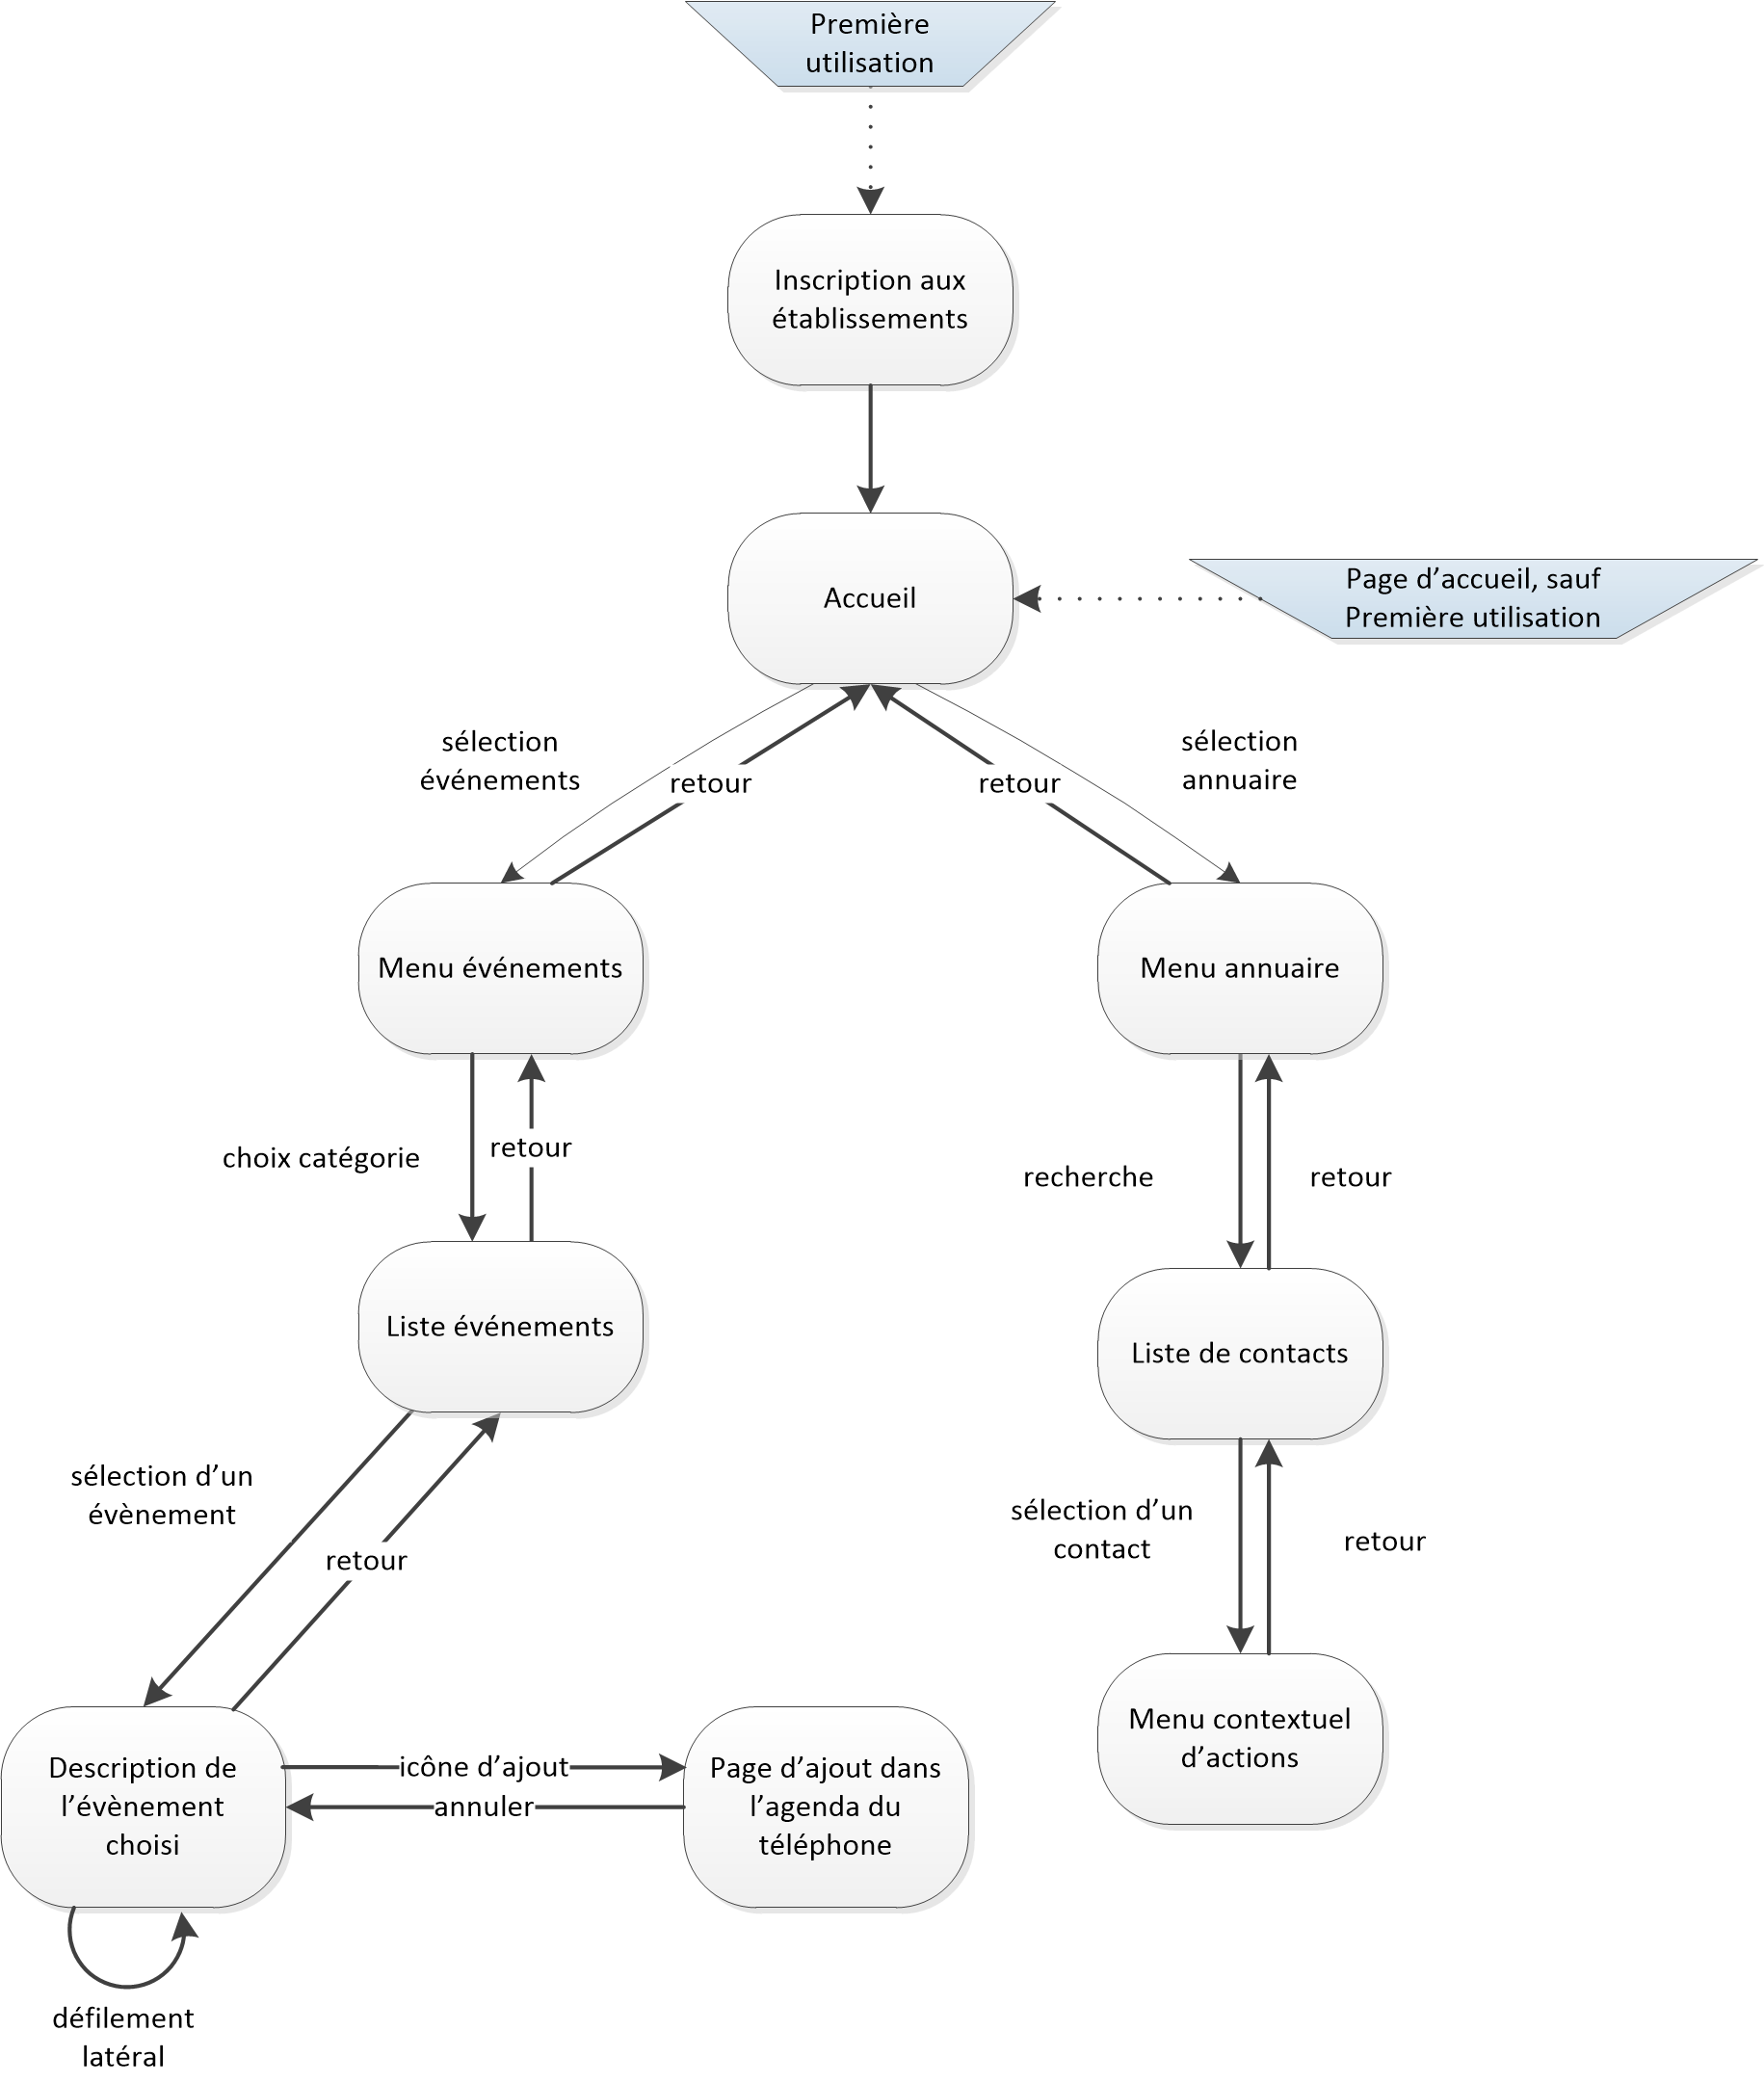
\includegraphics[width=0.75\textwidth]{resources/features1.png}
\end{figure}

\newpage

Le diagramme ci-dessus présente toutes les actions réalisables par l'utilisateur et leurs enchaînements.
Lorsque l'utilisateur démarre l'application pour la première fois, il choisit l'établissement auprès duquel il veut s'abonner.
Ce choix est alors retenu, et cette étape est donc omise lors des futurs démarrages de l'application. Une option existera tout de même pour modifier les abonnements si nécessaire. Depuis l'écran d'accueil, l'utilisateur pourra alors accéder aux services de son choix et pourra à tout moment revenir en arrière facilement. \\

\begin{figure}[h]
	\center
	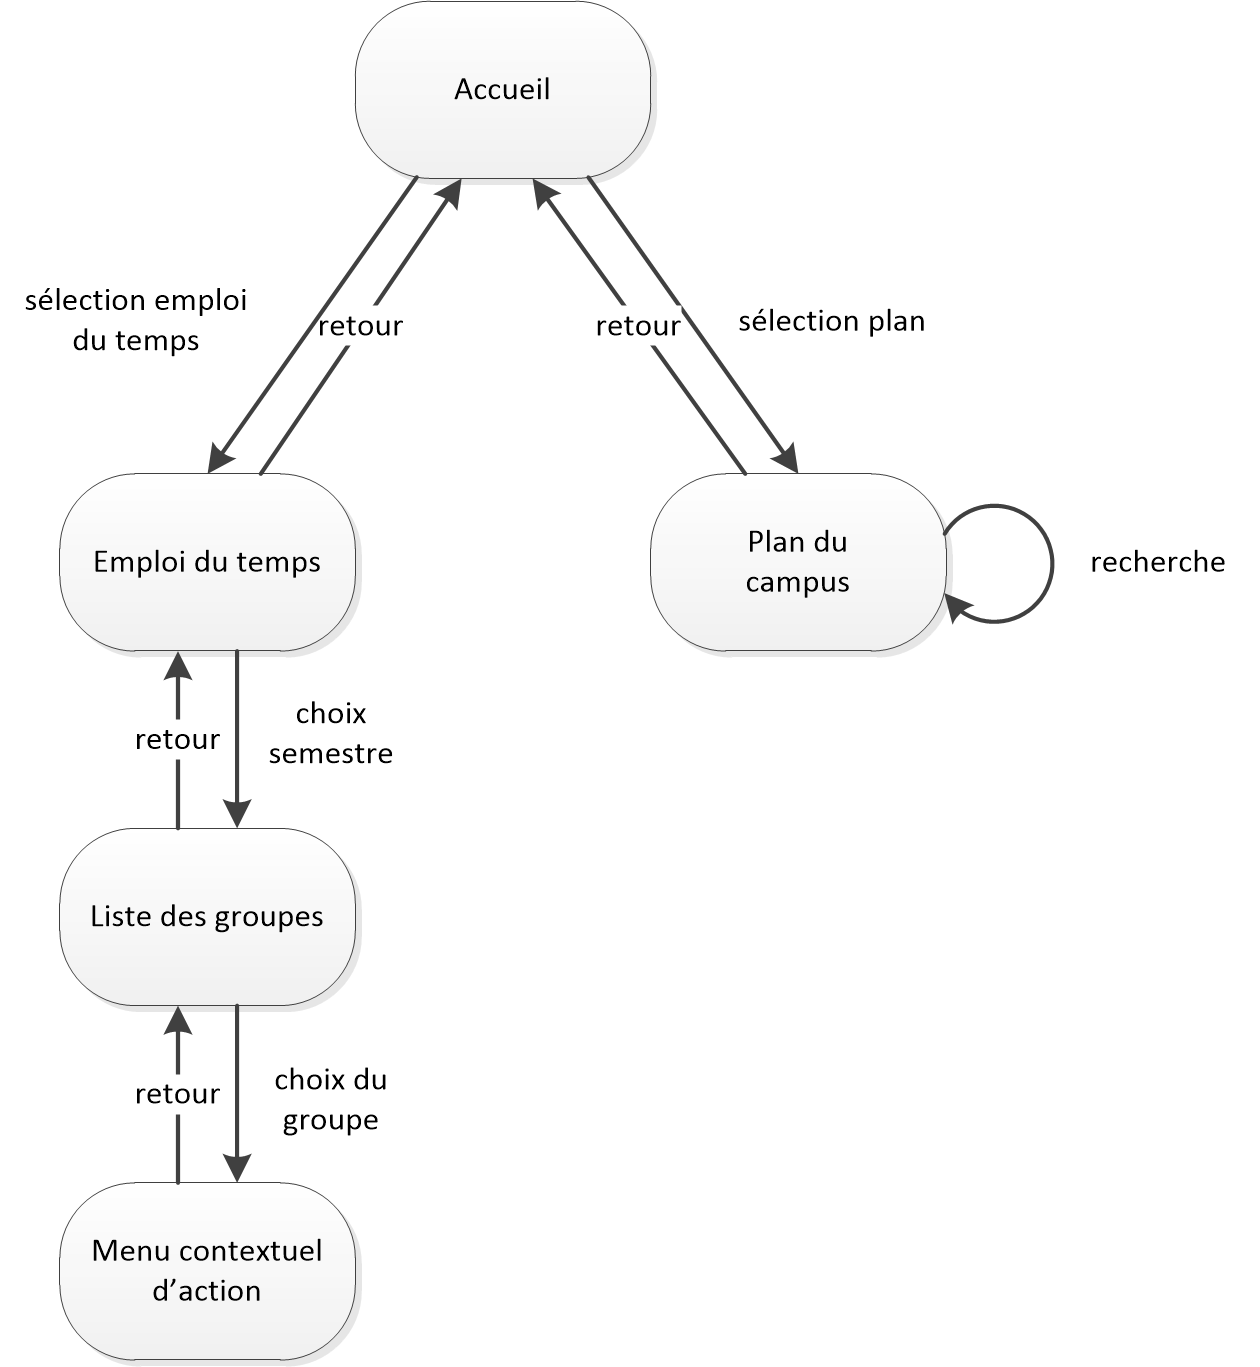
\includegraphics[width=0.65\textwidth]{resources/features2.png}
\end{figure}

Le diagramme ci-dessus présente les services offerts pour l'établissement Bordeaux1. Ces services supplémentaires seront implémentés après avoir assuré les fonctionnalités principales.

\newpage
\section{Diagramme des mises à jour}

\begin{figure}[h]
  \center
  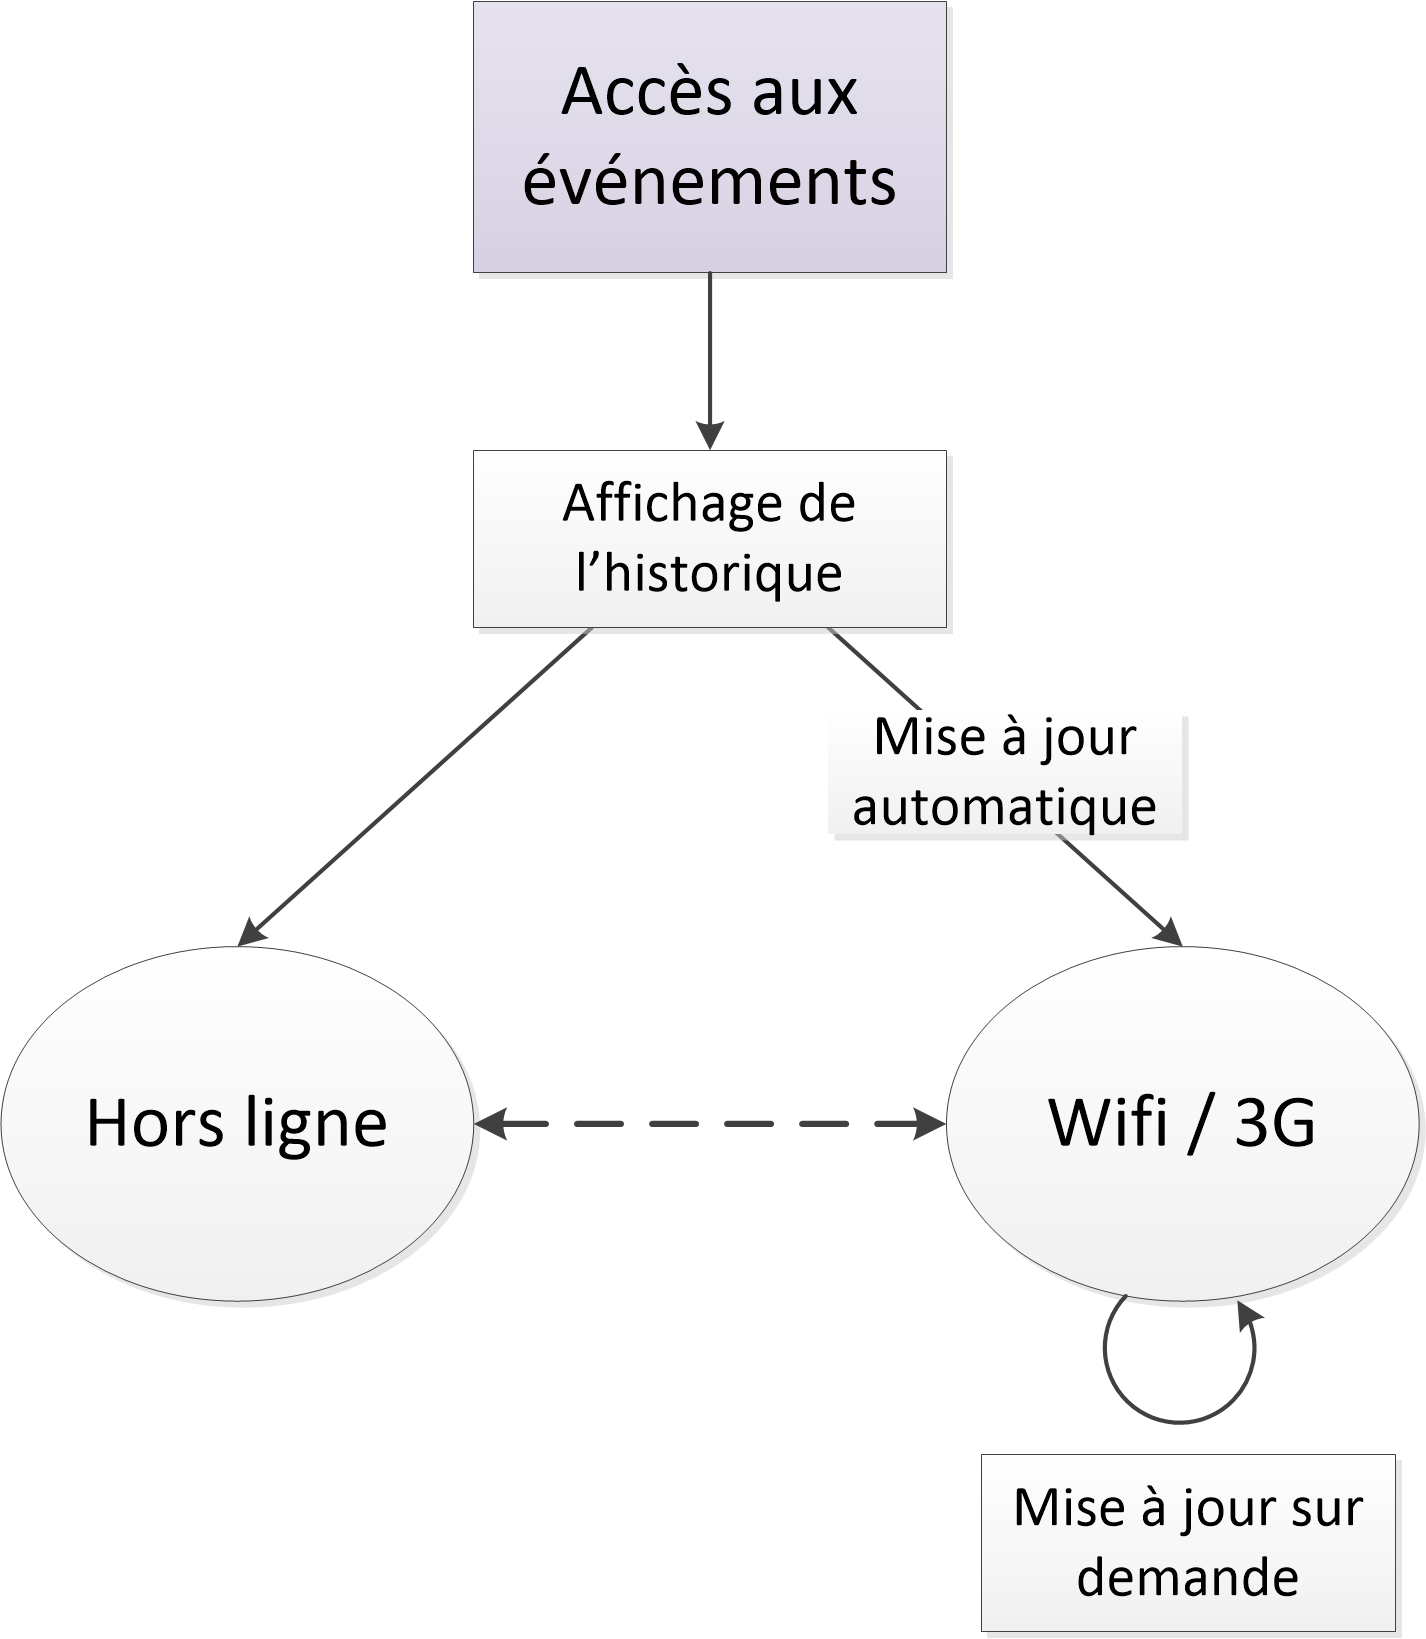
\includegraphics[width=0.5\textwidth]{resources/state_diagram.png}
\end{figure}

\wl Le diagramme de mises à jour représente les différents modes de connexion dans lesquels on peut se trouver lorsqu'on accède aux événements. Il y a trois modes possibles gérés par le téléphone :\\
\begin{itemize}
\renewcommand{\labelitemi}{$\bullet$}
 \item Hors Ligne : pas d'accès à Internet.
 \item 3G :  accès au réseau de données mobiles (lent).
 \item WiFi : accès à un réseau sans-fil (rapide).
\end{itemize}
